% !TEX root = ../thesis.tex
%\chapter{State of the Art}
\chapter{Technical Preliminaries}
\label{capitolo3}
\thispagestyle{empty}

\iffalse

This chapter discusses the state of the art that is relevant for your own work. What does that mean? It means that it provides the reader with all the relevant references he/she may need to know in order to understand better three things: (i) the context of your work, (ii) the problem and the need for a solution, and (iii) the value of your contribution. You achieve this by citing works or scientific papers that solved the same or similar problems in the past. Citing does not just mean adding a references to the bibliography and printing a number here; it means you tell the reader about the merits and possible demerits of each of the references you feel relevant. Of course, doing so requires you to first read each reference and, most importantly, to understand it. There should be lots of references in this chapter. 

It is advisable that you structure the chapter into sections in function of the topics you treat. If you do so, before starting with the first section of the chapter, explain the reader how you structure your discussion in one paragraph.

\begin{itemize}
\item[\Square] \emph{Read} relevant literature and or \emph{test} related software or tools.
\item[\Square] \emph{Summarize} your reading.
\item[\Square] Provide correct \emph{references} (the bibliography in the end of this document).
\end{itemize}

\fi


\section{Relational Database}
When dealing with computer systems, one of the most basic notions, often inappropriately taken for granted, is the one of ``\textbf{data}'', definable as:
\begin{quote}\emph{Information, especially facts or numbers, collected to be examined and considered and used to help decision-making, or information in an electronic form that can be stored and used by a computer.} \cite{cambridge2013data}\end{quote}
Therefore, a large amount of data stored in a computer in some organized manner is called a \textbf{database}. To be more precise, a database is ``any collection of data, or information, that is specially organized for rapid search and retrieval by a computer'' \cite{britannica2020database}; while the software that supports the management of these data is called a \textbf{database management system (DBMS)}.

The history of databases is deeply interconnected with the history of informatics itself, because the problem of how to store and retrieve information appeared as one of the initial challenges of computer creators. However, in the past few decades the rapid and enormous evolution of computer systems and databases led to the adoption and the development of the so called ``data models''. A \textbf{data model} is an abstract representation of an information system, which defines the data elements and the relationships between data elements. The aim of a data model is to give a clear and intuitive overview on how a system looks like, by providing a standardized description of its components, in such a way as to facilitate the understanding of the system itself and the possible integration with other systems.

Nowadays, the most widespread data model is the \textbf{relational model}, firstly proposed by E. F. Codd in \cite{codd1970relational}. The relational model represents a database as a collection of relations, depicted as tables of values. Each row of the table is a collection of related data values, referring to a real-world entity or relationship between entities. Therefore, we can simply define a \textbf{relational database} as a digital database based on the relational model of data.
To make it clearer, the following list provides the main terms used in this context, together with a concise explanation.
\begin{itemize}
\item \textbf{Table}, or \textbf{relation}: modeling of a real-world entity or of a relationship between real-world entities.
\item \textbf{Row}, or \textbf{tuple}: single data record.
\item \textbf{Column}, or \textbf{attribute}: property, or feature, of a relation.
\item \textbf{Cardinality}: total number of tuples of a relation.
\item \textbf{Degree}: total number of attributes of a relation.
\item \textbf{Primary key}: attribute, or combination of attributes, that uniquely identifies a tuple among the others.
\item \textbf{Domain}, or \textbf{data type}: set of values that a specific attribute can assume (for example, integer numbers or boolean values).
\item \textbf{Database schema}, or simply \textbf{schema}: blueprint of the database that outlines the way its structure organizes data into tables.
\item \textbf{Database instance}, or simply \textbf{instance}: set of tuples in which each tuple has the same number of attributes as one of the relations of the database schema. It specifies the actual content of the database.
\end{itemize} 

\begin{figure}[h!]
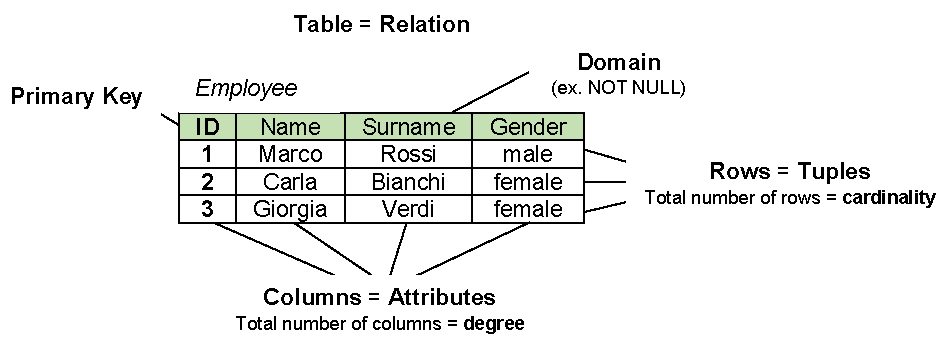
\includegraphics[scale=.75]{figures/relational_model.pdf}
\centering
\caption{Relational model concepts in a trivial example. ``Employee'' is the name of the real-world entity of reference and therefore of the related table in the model.}
\label{fig:relational_model}
\end{figure}

Lastly, since this term will be often used in the subsequent sections and chapters, we define a \textbf{dataset} as a collection of data. More specifically, since our data are in a tabular format according to the relational model, a dataset simply corresponds to one or more database tables.


\section{Data Science Pipeline}
Because of the broadness of the concept, there is not a unique and precise definition of data management. In general, we can identify it as the process of acquiring, storing, organizing, and maintaining data created and collected by an organization. In \cite{gandomi2015beyond}, the author, referring to \cite{labrinidis2012challenges}, classifies \textit{data management}, together with \textit{analytics}, as one of the two sub-processes to extract insights from data, while the overarching process is referred as \textbf{data science pipeline}. For the sake of clarity, since the term is the one used in \cite{gandomi2015beyond}, although it is not a concept strictly inherent to this research, we define big data as:
\begin{quote}
\emph{Large volumes of high velocity, complex and variable data that require advanced techniques and technologies to enable the capture, storage, distribution, management, and analysis of the information.} \cite{mills2012demystifying}\end{quote}
However we preferred to adopt the name of ``data science pipeline'' instead of ``big data pipeline'', since we will not deal with big data, which are not a concept strictly inherent to this research.

\begin{figure}[h!]
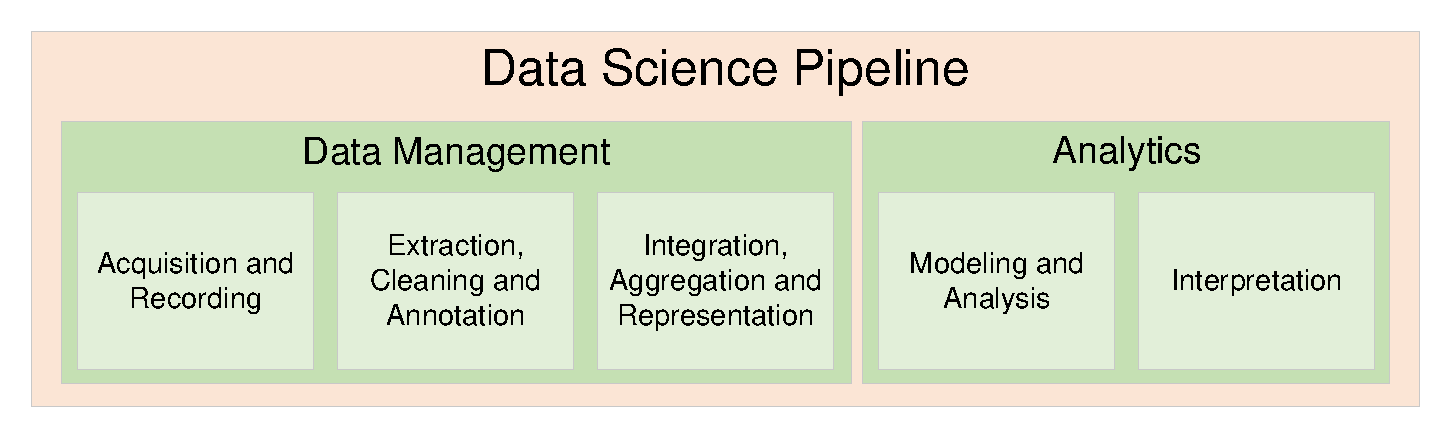
\includegraphics[scale=.5]{figures/data_science_pipeline.pdf}
\centering
\caption{Data science pipeline. Image based on the one shown in \cite{gandomi2015beyond}.}
\label{fig:data_science_pipeline}
\end{figure}

Since fairness should be addressed in each phase of the data science pipeline, the subsequent list provides a concise explanation of the operations performed in each step, by following the classification proposed in \cite{jagadish2014big}, together with the main potential sources of bias.
\begin{itemize}
\item \textbf{Acquisition and recording}: data are recovered and captured. In this phase the introduction of bias could derive from some preliminary critical choices we have to deal with, concerning the availability of sources, the identification of who is represented by the data, the definition of what has been measured and of our duties to the people in the data (for example, we may owe them a certain degree of privacy).
\item \textbf{Extraction, cleaning and annotation}: real data are most of the time messy and dirty, therefore we need to extract the relevant information and clean them, in order to express them in a structured form suitable for analysis. Unfortunately, data cleaning itself is based on assumptions, and wrong assumptions may lead to bias (for example, we may assume missing values in the data as missing at random, while there could be other, maybe ethical, reasons behind).
\item \textbf{Integration, aggregation and representation}: data analysis often requires the collection of heterogeneous data from different sources, therefore we need to integrate them in order to guarantee syntactic and semantic coherence. Again, we have to rely on assumptions on the world, as for the case of data representation, in which a lot of choices are made in order to decide what to represent, potentially leading to bias (for example, in the context of sentiment analysis we may ascribe sentiment to labels, or we may decide to group age values instead of considering every single year).
\item \textbf{Modeling and analysis}: before the actual analysis, an abstract model of the data is generated, in order to capture the essential components of the system and their interactions. However, the process of abstraction of concrete data in a conceptual standard model necessarily leads to the loss of information.
\item \textbf{Interpretation}: a decision-maker, provided with the results of the analysis, has to interpret these results. This process usually requires to examine all the assumptions made and to retrace the analysis, and because of the complexity of the task and the problems that may arise from computer systems (bugs, errors), a human (and therefore impossibly perfectly fair) supervision is needed.
\end{itemize}


\iffalse

Fairness requires social consensus.
Humans have many biases, no human is perfectly fair, even with the best of intentions.
Bias in algorithms in easier to detect than human bias, because humans are likely to defend their decisions with plausible explanations.
In machine learning, the past is assumed to be representative of the future (training, test); but in society this is often not true, because the world continuously change.

\textbf{Stability}: if you choose a different model, how likely is it that a small perturbation will result in a different answer?


\section{Summary}
Close the state of the art chapter with some words that connect the discussion of the references to your thesis. Pay attention that the reader understands why you discussed the works/topics you discussed and how they are related to what you do.

\begin{itemize}
\item[\Square] Show that in the state of the art the \emph{problem} you want to solve has not yet been solved or not been solved in an as efficient / effective / easy to use / cost-saving fashion as you target with your work.
\item[\Square] If your work has similarities with some \emph{specific references}, point them out here and explain why these are particularly important to you. Perhaps you started your investigation from the outputs of a specific paper or you want to improve the performance of an algorithm studied earlier; it's good to mention this here.
\item[\Square] Attention: this is not yet the place where to anticipate \emph{your solution}. You may give hints, but it's too early to make a comparison between your work and the state of the art, as the reader does not yet know anything about your work. This discussion can go into the final chapter.
\end{itemize}

\fi
